\documentclass[12pt]{article}

\usepackage[english]{babel}
\usepackage[utf8]{inputenc}
\usepackage[T1]{fontenc}
\usepackage{graphicx}
\usepackage{amsmath}
\usepackage{fancyhdr}
\usepackage{siunitx}
\usepackage{listings}

\makeatletter
\def\@seccntformat#1{\csname the#1\endcsname\hspace*{0.5em}$|$\hspace*{0.5em}}
\makeatother

\pagestyle{fancy}

\title{\textbf{Quartz resonator} \\ SCI-C0200}
\author{Joonatan Bergholm 507260 \\ Osama Abuzaid 524832}

\begin{document}

\pagenumbering{gobble}
\maketitle
\newpage

\pagenumbering{arabic}

\tableofcontents
\newpage

\section{Introduction}

\begin{figure}
	\centering
	\includegraphics[width = \textwidth]{kuvat/kvres.png}
	\caption{Quartz resonator.$^{\cite{Ohje}}$}
	\label{fig:kvres}
\end{figure}

In this assignment we investigated electronic properties of one of the most common electronic components, the quartz tuning fork or quartz resonator, like one in figure \ref{fig:kvres}. It is used in watches and other every day electrical appliances to provide a stable clocking frequency. Typically the frequency is $f_0 = \SI{32768}{\hertz}$, because is is a round number ($32768_{10} = {2^{15}}_{10} = 1000000000000000_2$) in base 2, which is commonly used in electrical appliances.

Contrary to conventional tuning fork, one does not need generate mechanical excitation
on the quartz tuning fork, because quartz has piezoelectric properties and thus mechanical excitation can be replaced with electronic one.$^{\cite{Intro}}$

\section{Tuning fork}
Piezoelectricity is a phenomena, where deformation of a material causes electrical current and vice versa. Crystal oscillators are made of piezoelectric materials, and in electric circuits they are used to produce an electrical signal with precise frequency. The Q-value of crystal oscillator is defined to be the oscillators energy per dissipated energy at one oscillation:
\begin{align}
Q \equiv 2\pi\frac{E}{\Delta E}.
\end{align}

In our work we are using quartz tuning forks. The fundamental frequency of a tuning fork is given by equation
\begin{align}
f_0 \approx 0.16\frac{T}{L^2}\sqrt{\frac{E}{\rho}},
\end{align}
where $L = 3.98 $mm is the length of one quartz bar, $T = 0.60 $mm the width of the bar, $E = 79 $GPa the Young modulus and $\rho = 2660\frac{\mathrm{kg}}{\mathrm{m}^3}$ the density of quartz. Also the thickness of fork we are using in our work is $H = 0.30$mm. Advantage of having two bars instead of one is that the oscillations of two bars at the fulcrum cancel each other, resulting to better Q-value.

We can estimate the Q-value of the tuning fork from figure \ref{fig:steady} by using equation$^{\cite{Qvalue}}$

\begin{align*}
t &= \frac{f_0}{Q}\\
\Rightarrow Q &= tf_0 \approx 13000
\end{align*}
where according to figure \ref{fig:steady} $t \approx 0.4$s is the time constant, which tells the time it takes for the resonator to stabilize to the equilibrium amplitude.

\begin{figure}[!ht]
\centering
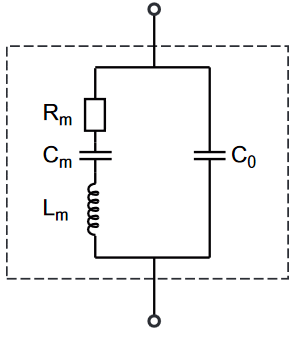
\includegraphics[width = 0.5\textwidth]{equivalence_circuit}
\caption{Equivalence circuit of a tuning fork.$^{\cite{Ohje}}$} \label{fig:equivalence_circuit}
\end{figure}

An equivalence circuit of tuning fork is an electrical circuit which can't be distinguished from tuning fork in a black box. The components of equivalence circuit in figure \ref{fig:equivalence_circuit} are obtained from following equations:
\begin{align} \label{eqn:equivalent}
\begin{cases}
L_m = \frac{2\rho L^3}{9e_p^2HT}\\
C_m = \frac{1}{\omega_0^2L_m}\\
R_m = \frac{\omega_0 L_m}{Q}=\gamma L_m\\
C_0 = \frac{\epsilon_0\epsilon_rA}{T}
\end{cases},
\end{align}
where $e_p \approx 0.18 \frac{\mathrm{C}}{\mathrm{m}^2}$ is the piezoelectric modulus of tuning fork, $\epsilon_0$ and $\epsilon_r$ are the vacuum and relative permittivity, respectively, and $A = TL$ the effective area. Equivalence circuit of our tuning fork would have following components:
\begin{align*}
\begin{cases}
L_m \approx 3.3\cdot10^{-20}~\mathrm{H}\\
C_m \approx 7.1\cdot10^8~\mathrm{F}\\
R_m \approx 5.3\cdot10^{-19}~\Omega\\
C_0 \approx 3.5\cdot10^{-9}~\mathrm{F}
\end{cases}
\end{align*}

As we can see, the values are far from typical, so it would be very difficult and expensive to produce needed components.

\begin{figure}
	\centering
	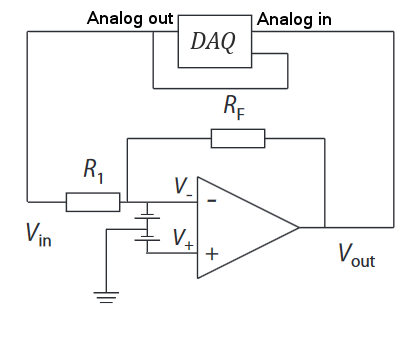
\includegraphics[width = 0.5\textwidth]{kuvat/piiri}
	\caption{Circuit used to collect data. Both batteries are 9V.}
	\label{fig:circuit}
\end{figure}

\begin{figure}[!ht]
	\centering
	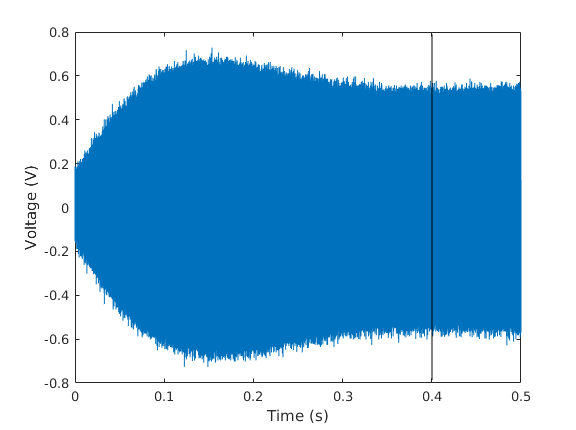
\includegraphics[width = \textwidth]{kuvat/steadystate.png}
	\caption{Voltage plotted from connecting the driving voltage to $\SI{0.5}{\second}$ after connecting.}
	\label{fig:steady}
\end{figure}

\section{Our circuit}

The circuit we made and used is basically a voltage amplifier built around LF356N operational amplifier with two resistors ($ R_1 = \SI{1}{\kilo\ohm}$ and $R_f = \SI{10}{\kilo\ohm}$) and later it is modified to current-voltage converter by replacing $R_1$-resistor with quartz resonator and changing $R_f$-resistor to a approximately $\SI{1}{\mega\ohm}$-resistor. The derivation of transresistance $K$ (equation \eqref{eqn:K}) is done in the appendix as part of a pretask.

First we characterised the circuit by measuring its $G$-value by altering input voltage within range $\SI{0}{\volt} - \SI{1.7}{\volt}$ and reading the output voltage for each input voltage. Theoretical value is $G = -\frac{R_f}{R_1} \approx 10$ and with our measurement we obtained $G \approx 10.2$, which is quite good considering that usually resistors have 5\% - 10\% error margins in their values. According to this experiment a good amplitude for input voltage in ac-measurements would be something like $\SI{0.2}{\volt} - \SI{0.6}{\volt}$, because our circuit can only amplify signal up to $\SI{9}{\volt}$. Both for ac and dc, because ac for short periods of time is like dc, and thus our circuit amplifies them the same, except that there might some kind of echo effect or the circuit has a reaction time, because for high frequency ac the output has high amount of noise.

To measure quartz resonator the circuit must be connected to a DAQ-unit as shown in figure \ref{fig:circuit} and then it can be measured by setting the DAQ-unit to output a sine wave with certain frequency and then measuring the output of our circuit. With multiple measurements a spike in gain is expected at the resonance frequency of the quartz resonator as seen in figure \ref{fig:f-g}. Also as seen in figure \ref{fig:f-ps_res} the phase shift seems to go towards $\pi$ when the frequency goes towards resonance frequency.

We tested our circuit at frequency range of $\SI{10}{\kilo\hertz} - \SI{100}{\kilo\hertz}$ and noticed that the noise increases with the frequency, but however at approximately $\SI{30}{\kilo\hertz}$ the noise-to-signal ratio is still reasonable as seen in figure \ref{fig:nsr}, so we can use our circuit to obtain quite good approximations of properties of quartz resonator. The same noise is seen in figure \ref{fig:f-ps}.$^\cite{Ohje}$

\begin{figure}[!ht]
\centering
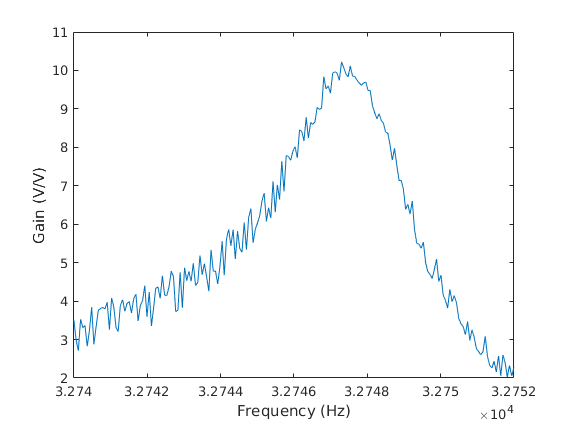
\includegraphics[width = 0.8\textwidth]{kuvat/f-g.png}
\caption{Gain in circuit as function of frequency. Spike is clearly seen at resonance frequency of the resonator.}
\label{fig:f-g}
\end{figure}

\begin{figure}[!ht]
\centering
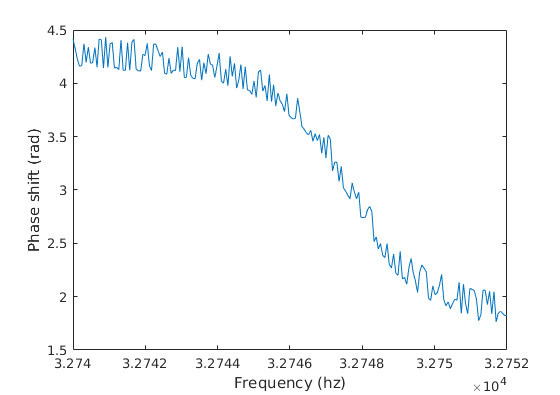
\includegraphics[width = 0.8\textwidth]{kuvat/f-ps_res.png}
\caption{Phase shift in circuit as function of frequency near resonance frequency.}
\label{fig:f-ps_res}
\end{figure}

%\begin{figure}[!ht]
%\centering
%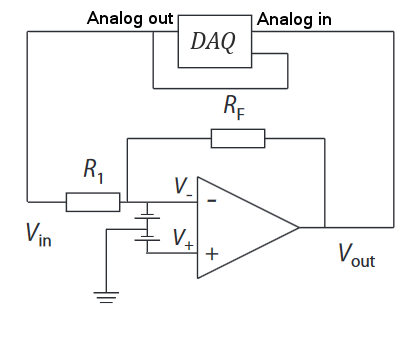
\includegraphics[width = \textwidth]{kuvat/piiri.png}
%\caption{Circuit diagram of voltage amplifier connected to DAQ-unit.}
%\label{fig:circ}
%\end{figure}

\begin{figure}[!ht]
\centering
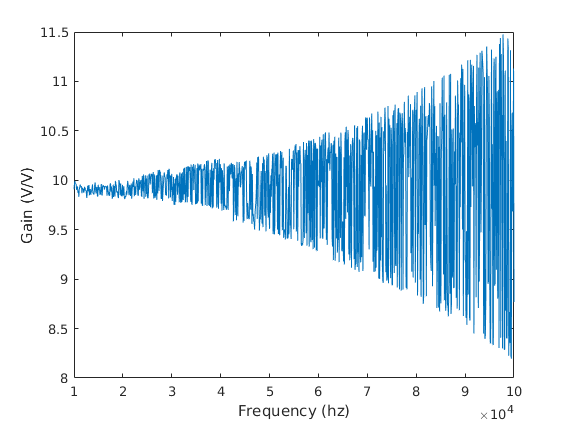
\includegraphics[width = 0.8\textwidth]{kuvat/nsr.png}
\caption{Gain as function of frequency without quartz resonator.}
\label{fig:nsr}
\end{figure}

\begin{figure}[!ht]
\centering
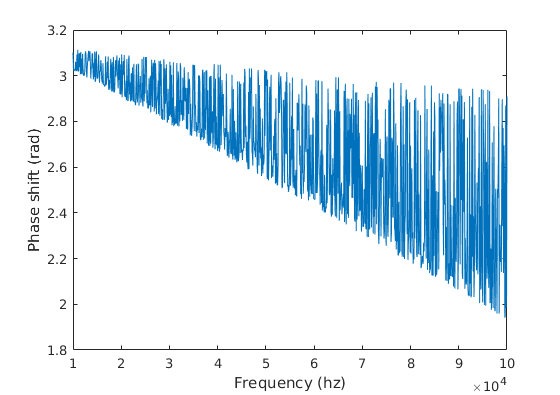
\includegraphics[width = 0.8\textwidth]{kuvat/f-ps.png}
\caption{Phase shift as function of frequency.}
\label{fig:f-ps}
\end{figure}

\newpage

\begin{thebibliography}{1}
\bibitem{Intro} \texttt{https://mycourses.aalto.fi/pluginfile.php/211815/mod\_folder\\/content/0/TuningFork.pdf}, "Introduction to the quartz tuning fork", accessed 2016.06.01

\bibitem{Ohje} \texttt{https://mycourses.aalto.fi/pluginfile.php/211815/mod\_resource\\/content/1/projekti\_tyoohjeet.pdf}, "SCI-C0200 Fysiikan ja matematiikan menetelmien studio (10 op)
Projektityö: Kvartsikiteen ominaisvärähtelyn mittaus ja analysointi, Työn taustamateriaali", accessed 2016.06.01

\bibitem{Qvalue} \texttt{https://mycourses.aalto.fi/pluginfile.php/211810/mod\_resource\\/content/1/projekti\_kertaohje4.pdf}, "Kvartsiresonaattorin mittaus", accessed 2016.06.01
\end{thebibliography}

\newpage
\appendix

\section{Source code}

\lstinputlisting[caption = ac.m]{matlab/ac.m}
%\lstinputlisting[caption = ac.m]{matlab/DAQreadout.m}

\section{Pretasks}

\subsection{Session 1}

\subsubsection{Task 1}

In this project we are supposed to study electric properties of quartz resonators and build a circuit, which is used to collect data from the resonator. Data is then analyzed with MATLAB. Also we are going to measure some properties of the circuit itself.

\subsubsection{Task 2} \label{sec:voltamp}

$V_+$ is connected to ground, so $V_+ = 0$.

\begin{align*}
V_{out} =& A(V_+ - V_-) \\
\Rightarrow V_{out} =& -AV_-
\end{align*}

Then according to Kirchoff II and Ohm's law,

\begin{align*}
V_- - V_{out} = R_f I \quad \wedge & \quad I = \frac{V_{in} - V_{out}}{R_f + R_{in}} \\
\Rightarrow V_- =& R_f \frac{V_{in} - V_{out}}{R_f + R_{in}} + V_{out} \\
\Rightarrow V_- =& \frac{R_f V_{in} - R_f V_{out}}{R_f + R_{in}} + \frac{R_f V_{out} + R_{in} V_{out}}{R_f + R_{in}} \\
\Rightarrow V_- &= \frac{R_f V_{in} + R_{in} V_{out}}{R_f + R_{in}} \\
\end{align*}

Then combining these two equations, we obtain $V_{out}$ as function of $V_{in}$.

\begin{align*}
V_{out} &= -A\frac{R_f V_{in} + R_{in} V_{out}}{R_f + R_{in}} \\
\Leftrightarrow V_{out} + A\frac{R_{in} V_{out}}{R_f + R_{in}} &= -\frac{A R_f V_{in}}{R_f + R_{in}} \\
\Leftrightarrow V_{out}\frac{R_f + R_{in} + A R_{in}}{R_f + R_{in}} &= -\frac{A R_f V_{in}}{R_f + R_{in}} \\
\Leftrightarrow V_{out} &= -\frac{A R_f}{R_f + R_{in} + A R_{in}} V_{in}
\end{align*}

When $A$ is very large, we obtain the following form.

\begin{equation*}
V_{out} \approx -\frac{R_f}{R_{in}} V_{in}
\end{equation*}

And thus,

\begin{equation}
G = -\frac{R_f}{R_{in}}
\label{eqn:G}
\end{equation}

\subsection{Session 2}

\subsubsection{Task 2}

In old western movies the wagon wheel seems to be rotating in the wrong direction because camera's frame rate is so slow that it can't properly get samples of fast rotating wagon wheel, and thus the rods have enough time between frames to move in positions that are closer to the next rod's previous position than rod's original position.

\subsubsection{Task 3}

As seen in figure \ref{fig:samp} the higher the frequency of the signal is the worse the samples fit to signal. Thus with $\SI{10}{\kilo\hertz}$ signal the samples show the shape correctly, but with $\SI{250}{\kilo\hertz}$ signal they do not.

\begin{figure}[!ht]
\centering
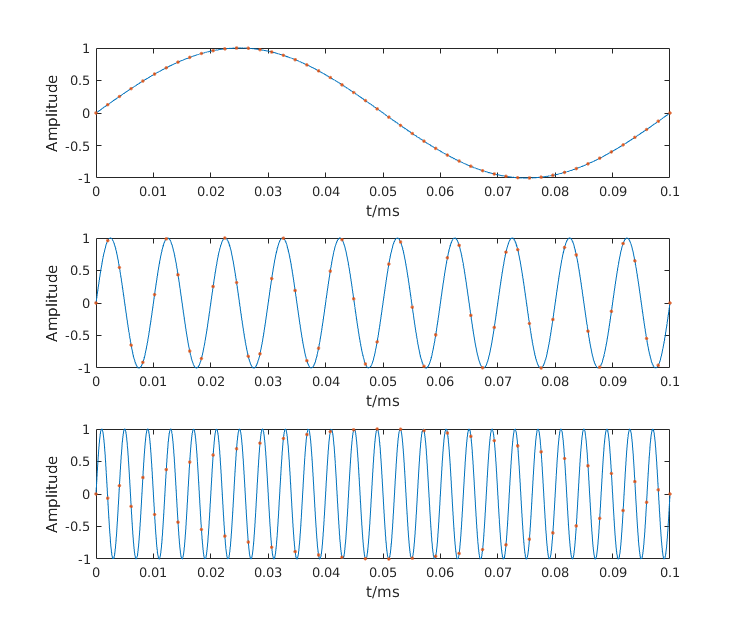
\includegraphics[width = \textwidth]{kuvat/sampling.png}
\caption{Sine waves (blue) and samples (red) for frequencies $\SI{10}{\kilo\hertz}$, $\SI{100}{\kilo\hertz}$ and $\SI{250}{\kilo\hertz}$ with sampling frequency of $\SI{500}{\kilo\hertz}$.}
\label{fig:samp}
\end{figure}

\subsubsection{Task 4}

Tasks 2 and 3 are actually the same phenomenon, where sampling frequency affects the collected data and thus may make it seem like something else than it is.

\subsection{Session 3}

\subsubsection{Task 1}

Let signal $s(t) = A \sin (2\pi(nf_s \pm f_1) \cdot t)$, where sampling frequency is $f_s$ and thus after sampling we only take values of $t$ which conform equation $t = k/f_s$, where $k = 0, 1, 2, 3...$ Thus the sampled signal $s_s$ is

\begin{align*}
s_s(k) &= A \sin (2\pi k \cdot (n \pm \frac{f_1}{f_s})) \\
&= A \sin (2\pi kn \pm 2\pi k \frac{f_1}{f_s}) \\
&= A (\sin (2\pi kn) \cos (\pm 2\pi k \frac{f_1}{f_s}) + \sin (\pm 2\pi k \frac{f_1}{f_s}) \cos (2\pi kn)) \\
&= A \sin (\pm 2\pi k \frac{f_1}{f_s}) \\
&= A \sin (\pm 2\pi f_1 t)
\end{align*}

Thus sampled signal of $s$ looks the same as signal with frequency $f_1$.

\subsubsection{Task 2}

According to Kirchoff's laws and basic operational amplifier properties,

\begin{align*}
V_- - V_{out} = R_f I_{in} \quad & \wedge \quad V_{out} = -AV_- \\
\Rightarrow -V_{out} (1 + \frac{1}{A}) &= R_f I_{in} \\
\Leftrightarrow V_{out} &= -\frac{A}{A + 1} R_f I_{in}
\end{align*}

And because $A$ is usually large,

\begin{equation*}
I_{in} \approx \frac{V_{out}}{R_f}
\end{equation*}

\subsubsection{Task 3} \label{sec:K}
According to previous task,

\begin{align}
V_{out} &= -R_f I_{in} \notag \\
\Rightarrow K &= -R_f
\label{eqn:K}
\end{align}

Thus our circuit works as a current-voltage converter.

\subsubsection{Task 4}

A good voltage meter must have a high impedance, because then it doesn't create an alternate route for current and thus affects the circuit as little as possible.

A good current meter on the other hand must have a low impedance, because it must let current flow through itself, and if it has a high impedance it affects the flow of current.


\subsubsection{Task 5}
With trasimpedance amplifier it is possible to have a big voltage even with small currents, which makes measurements more easy and accurate. If we used a resistance instead, the voltage after it would be at most the same as before, meaning we would need more accurate measurement instruments to obtain the same accuracy.

\subsection{Session 4}

\subsubsection{Task 1}

Let stone be a cube length of a side $d = \SI{0.1}{\metre}$.

\begin{align*}
C = \epsilon \frac{A}{d} = \epsilon d \quad \wedge \quad Q &= CU \quad \wedge \quad \frac{Q}{d^2} = e_p \frac{x}{d} \\
\Rightarrow \frac{\epsilon d U}{d} &= e_p x \\
\Leftrightarrow U &= \frac{e_p x}{\epsilon}
\end{align*}

Also $F = \frac{EAx}{d} = Edx$, thus

\begin{equation*}
U = \frac{e_p F}{\epsilon_0 \epsilon_r E d}
\end{equation*}

Assuming some values $E = \SI{79}{\giga\pascal}$, $e_p = \SI{0.18}{\coulomb\per\square\meter}$, $F = \SI{500}{\newton}$, $\epsilon_r = 4.5$ and $\epsilon_0 \approx \SI{9e-12}{\farad\per\meter}$ we obtain

\begin{equation*}
U \approx \SI{280}{\volt}
\end{equation*}


\subsubsection{Task 2}

To fit to hand the length of tuning fork must be $l \approx \SI{0.1}{\meter}$ and usually they are made of steel which has density $\rho \approx \SI{7.7e3}{\kilo\gram\per\cubic\meter}$ and young's modulus $E = \SI{200}{\giga\pascal}$. Also they have frequency $f_0 = \SI{440}{\hertz}$. We solve $T$ from equation $f_0 \approx 0.16 \frac{T}{L^2} \sqrt{\frac{E}{\rho}}$ and obtain

\begin{equation*}
T = \frac{f_0 L^2}{0.16} \sqrt{\frac{\rho}{E}} \approx \SI{0.5}{\centi\meter}
\end{equation*}

The result for thickness $T$ is reasonable, so it is possible to build tuning fork with these characteristics.


\subsubsection{Task 3}

We use sampling frequency of $\SI{500}{\kilo\hertz}$, which is over two times as large as signal frequency $\SI{33}{\kilo\hertz}$, so according to 2. session's pretasks it should be easily usable for this measurement.

\subsection{Session 5}

\subsubsection{Task 1}
Substituting the values to the \eqref{eqn:equivalent} we find the values for the equivalent circuit to be

\begin{align*}
\begin{cases}
L_m \approx 3.3\cdot10^{-20}~\mathrm{H}\\
C_m \approx 7.1\cdot10^8~\mathrm{F}\\
R_m \approx 5.3\cdot10^{-19}~\Omega\\
C_0 \approx 3.5\cdot10^{-9}~\mathrm{F}
\end{cases}
\end{align*}
\subsubsection{Task 2}
Impedance of the equivalent circuit is given by equation
\begin{align*}
Z(\omega)^{-1} = i\omega C_0 + \left(R_m+\frac{1}{i\omega C_m} + i\omega L_m \right)^{-1}.
\end{align*}
Assuming $C_0=0$ and using \eqref{eqn:equivalent} we can simplify this:
\begin{align*}
Z(\omega) &= R_m+\frac{1}{i\omega C_m} + i\omega L_m\\
&=\gamma L_m+\frac{1}{i\omega \frac{1}{\omega_0^2L_m}} + i\omega L_m\\
&=\frac{L_m}{\omega}\left[\gamma\omega + i\left(\omega^2 - \omega_0^2\right)\right]
\end{align*}
The modulus of impedance is then
\begin{align} \label{eqn:impedance}
\left| Z(\omega) \right| = \frac{L_m}{\omega}\sqrt{\gamma^2\omega^2 +\left(\omega^2 - \omega_0^2\right)^2}
\end{align}

\subsection{Task 3}
Ohms law gives $I = \frac{U}{|Z|}$, and substituting \ref{eqn:impedance} to $|Z|$ we get
\begin{align}
	I(\omega) = \frac{U\omega}{L_m\sqrt{\gamma^2\omega^2 +\left(\omega^2 - \omega_0^2\right)^2}}.
\end{align}
When $\omega \approx \omega_0$, by using \eqref{eqn:equivalent} we obtain
\begin{align*}
	I(\omega) &\approx \frac{U\omega_0}{L_m}\frac{1}{\sqrt{\gamma^2\omega^2 +\left(\omega^2 - \omega_0^2\right)^2}}\\
	&=\frac{U\omega_0}{\frac{2\rho L^3}{9e_p^2HT}}\frac{1}{\sqrt{\gamma^2\omega^2 +\left(\omega^2 - \omega_0^2\right)^2}}\\
	&=\frac{(9/2)U\omega_0e_p^2HT}{\rho L^3}\frac{1}{\sqrt{\gamma^2\omega^2 +\left(\omega^2 - \omega_0^2\right)^2}}\\
	&=\frac{F}{m}\frac{1}{\sqrt{\gamma^2\omega^2 +\left(\omega^2 - \omega_0^2\right)^2}},
\end{align*}

where $F = \frac{9}{2}U\omega_0e_p^2HT$ and $m = \rho L^3$. Thus the current as a function of frequency is the general form of a driven harmonic oscillator.
\end{document}
